% Options for packages loaded elsewhere
\PassOptionsToPackage{unicode}{hyperref}
\PassOptionsToPackage{hyphens}{url}
%
\documentclass[
  11pt,
]{article}
\usepackage{amsmath,amssymb}
\usepackage[]{mathpazo}
\usepackage{iftex}
\ifPDFTeX
  \usepackage[T1]{fontenc}
  \usepackage[utf8]{inputenc}
  \usepackage{textcomp} % provide euro and other symbols
\else % if luatex or xetex
  \usepackage{unicode-math}
  \defaultfontfeatures{Scale=MatchLowercase}
  \defaultfontfeatures[\rmfamily]{Ligatures=TeX,Scale=1}
\fi
% Use upquote if available, for straight quotes in verbatim environments
\IfFileExists{upquote.sty}{\usepackage{upquote}}{}
\IfFileExists{microtype.sty}{% use microtype if available
  \usepackage[]{microtype}
  \UseMicrotypeSet[protrusion]{basicmath} % disable protrusion for tt fonts
}{}
\makeatletter
\@ifundefined{KOMAClassName}{% if non-KOMA class
  \IfFileExists{parskip.sty}{%
    \usepackage{parskip}
  }{% else
    \setlength{\parindent}{0pt}
    \setlength{\parskip}{6pt plus 2pt minus 1pt}}
}{% if KOMA class
  \KOMAoptions{parskip=half}}
\makeatother
\usepackage{xcolor}
\usepackage[margin=1in]{geometry}
\usepackage{graphicx}
\makeatletter
\def\maxwidth{\ifdim\Gin@nat@width>\linewidth\linewidth\else\Gin@nat@width\fi}
\def\maxheight{\ifdim\Gin@nat@height>\textheight\textheight\else\Gin@nat@height\fi}
\makeatother
% Scale images if necessary, so that they will not overflow the page
% margins by default, and it is still possible to overwrite the defaults
% using explicit options in \includegraphics[width, height, ...]{}
\setkeys{Gin}{width=\maxwidth,height=\maxheight,keepaspectratio}
% Set default figure placement to htbp
\makeatletter
\def\fps@figure{htbp}
\makeatother
\setlength{\emergencystretch}{3em} % prevent overfull lines
\providecommand{\tightlist}{%
  \setlength{\itemsep}{0pt}\setlength{\parskip}{0pt}}
\setcounter{secnumdepth}{-\maxdimen} % remove section numbering
\ifLuaTeX
  \usepackage{selnolig}  % disable illegal ligatures
\fi
\usepackage[]{natbib}
\bibliographystyle{plainnat}
\IfFileExists{bookmark.sty}{\usepackage{bookmark}}{\usepackage{hyperref}}
\IfFileExists{xurl.sty}{\usepackage{xurl}}{} % add URL line breaks if available
\urlstyle{same} % disable monospaced font for URLs
\hypersetup{
  pdftitle={Results parrot mimicry},
  hidelinks,
  pdfcreator={LaTeX via pandoc}}

\title{Results parrot mimicry}
\author{}
\date{\vspace{-2.5em}November 11, 2022}

\begin{document}
\maketitle

We scored the vocal mimicry ability of 398 species (for the full
distribution see Figure 1). 137 of showed at least one mimic. {[}Do we
want to say something about the ancestral state reconstrution depicted
in Figure 1?{]}

\begin{figure}
\centering
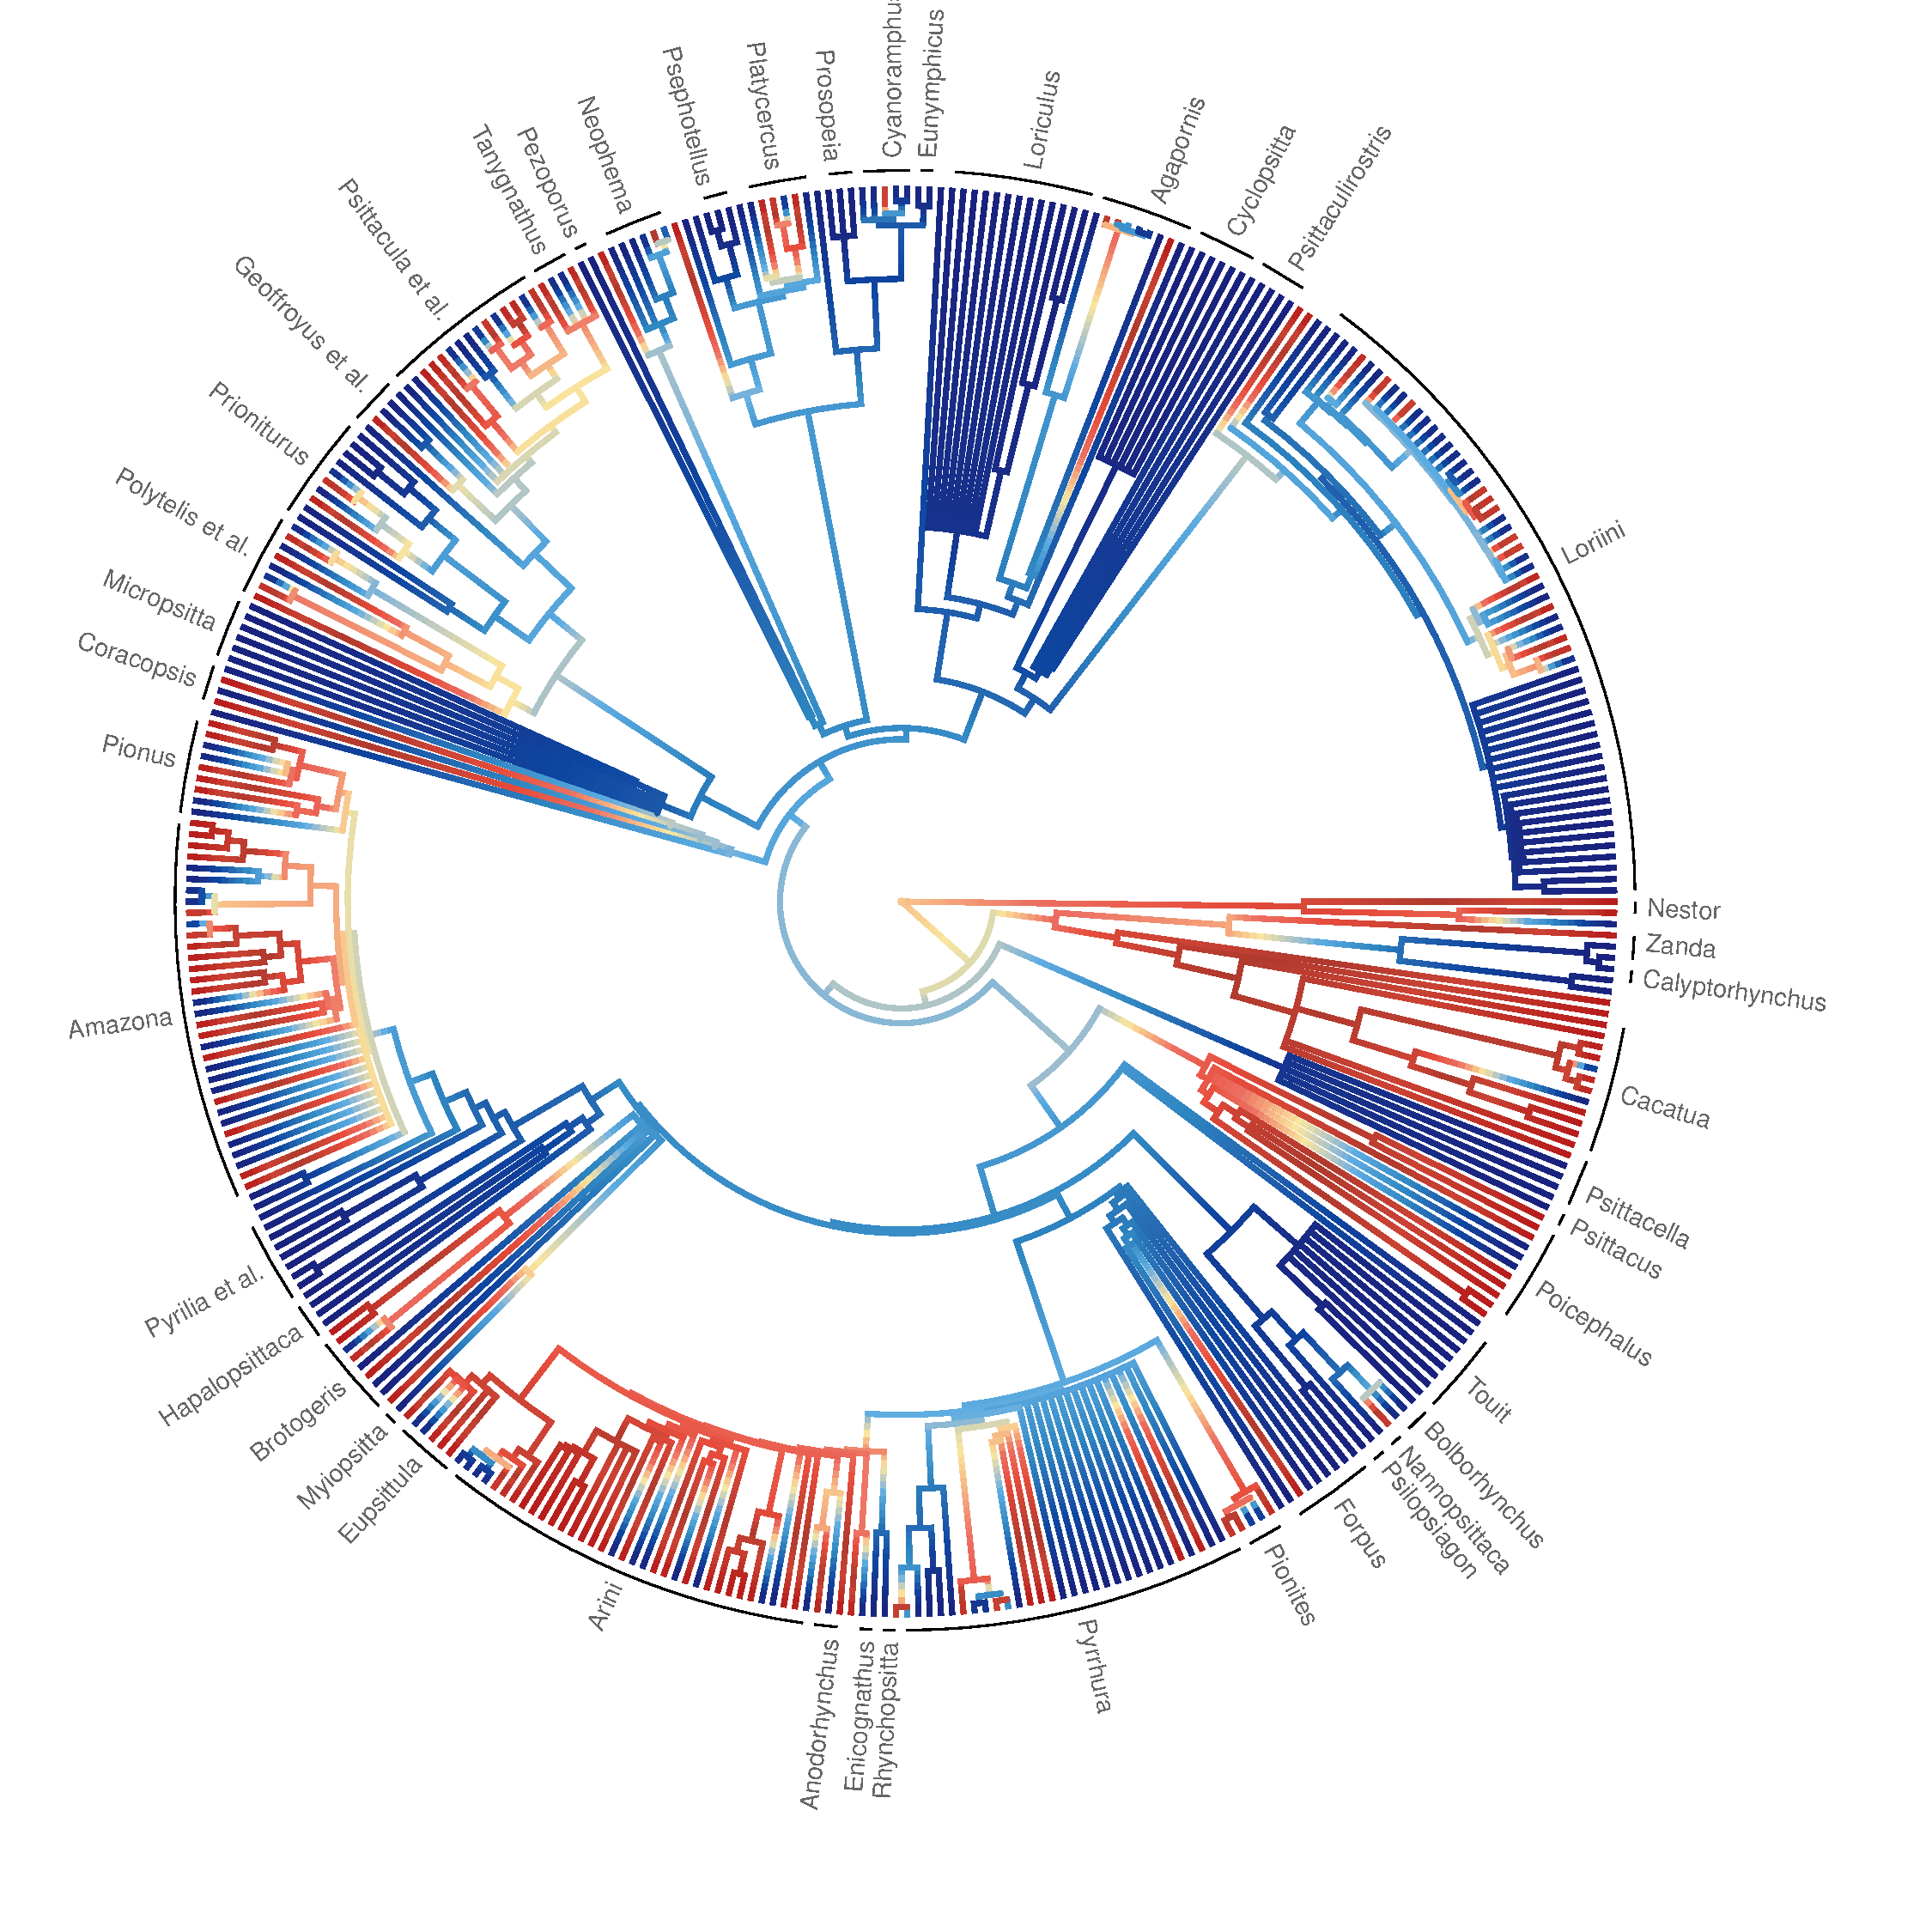
\includegraphics{/Users/ssmeele/ownCloud/Simeon/MPI AB/Side projects/Parrort mimicry/parrot_mimicry/ANALYSIS/RESULTS/tree mimicry or not.pdf}
\caption{Phylogenetic tree of all parrots species for which vocal
mimicry was assessed. Colours represent the ancestral state
reconstruction of vocal mimicry ranging from blue = no vocal mimicry
detected to red = vocal mimicry detected.}
\end{figure}

We ran four models to test the total effect of longevity, relative brain
size, sociality and body size on the probability that a species can
mimic. All variables had a positive total effect, although the effect of
relative brain size was highly uncertain (see Figure 2).

\begin{figure}
\centering
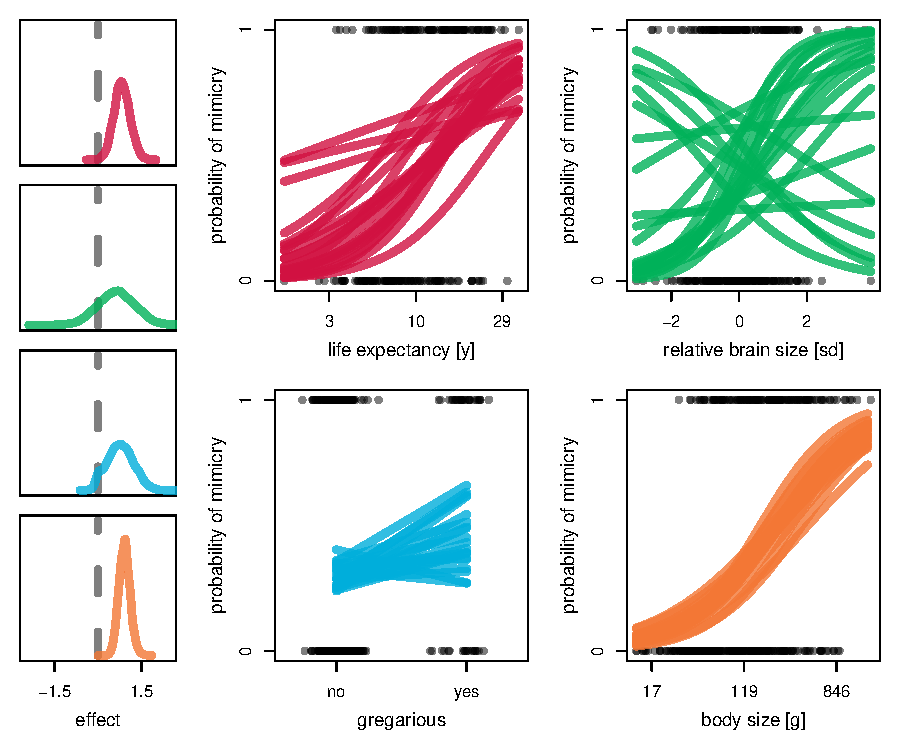
\includegraphics{/Users/ssmeele/ownCloud/Simeon/MPI AB/Side projects/Parrort mimicry/parrot_mimicry/ANALYSIS/RESULTS/results presence mimicry.pdf}
\caption{Variables influencing the probability of a species being able
to mimic. Lefthand side: posterior densities of the effect of longevity
(red), relative brain size (green), gregariousness (blue) and body size
(orange). For gregariousness the contrast between a non-gregarious and a
gregarious species is shown. For all other variables the slope is shown.
Righthand side: scatterplots of the raw data (grey) and 20 posterior
predictions (coloured lines) per variable.}
\end{figure}

We recorded the number of unique mimics that an individual produced for
843 individuals across 136 species. We ran four models to test the total
effect of longevity, relative brain size, sociality and body size on the
number of unique mimics that an individual produced in a video.
Longevity had no effect, relative brain size had a highly uncertain
effect, while sociality and body size had a small positive effect (see
Figure 3).

\begin{figure}
\centering
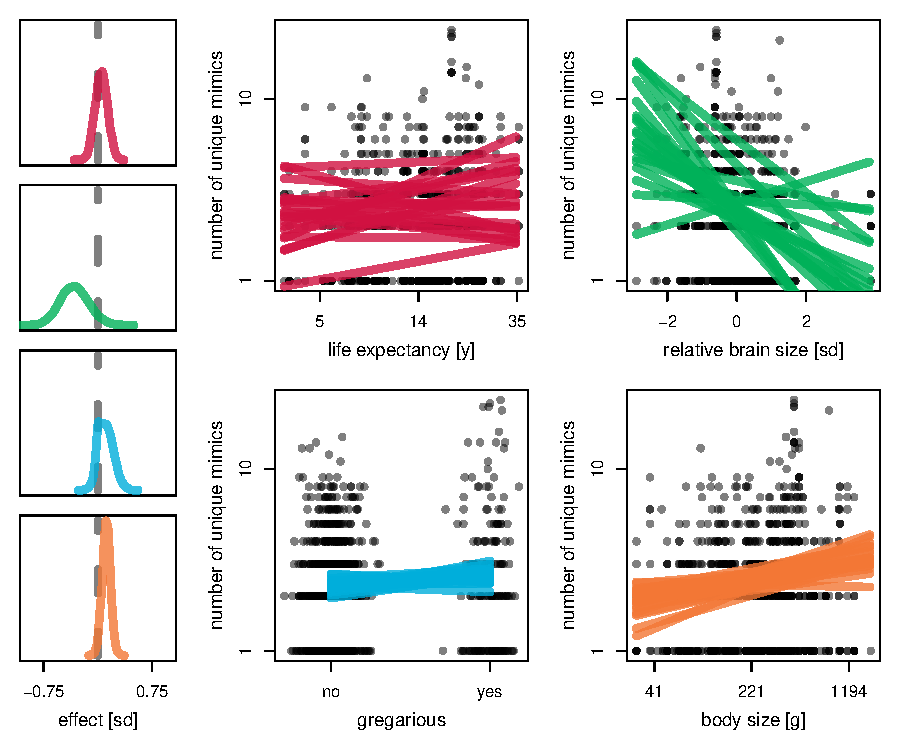
\includegraphics{/Users/ssmeele/ownCloud/Simeon/MPI AB/Side projects/Parrort mimicry/parrot_mimicry/ANALYSIS/RESULTS/results number of unique mimics.pdf}
\caption{Variables influencing the number of mimics an individual
produced in a video. Lefthand side: posterior densities of the effect of
longevity (red), relative brain size (green), gregariousness (blue) and
body size (orange). For gregariousness the contrast between a
non-gregarious and a gregarious species is shown. For all other
variables the slope is shown. Righthand side: scatterplots of the raw
data (grey) and 20 posterior predictions (coloured lines) per variable.}
\end{figure}

We also tested the influence of the four variable on the unique number
of words an individual produced in a video (see Figure 4). Longevity had
a clear total effect. Relative brain size had no clear effect. Sociality
and body size had a small and uncertain effect.

\begin{figure}
\centering
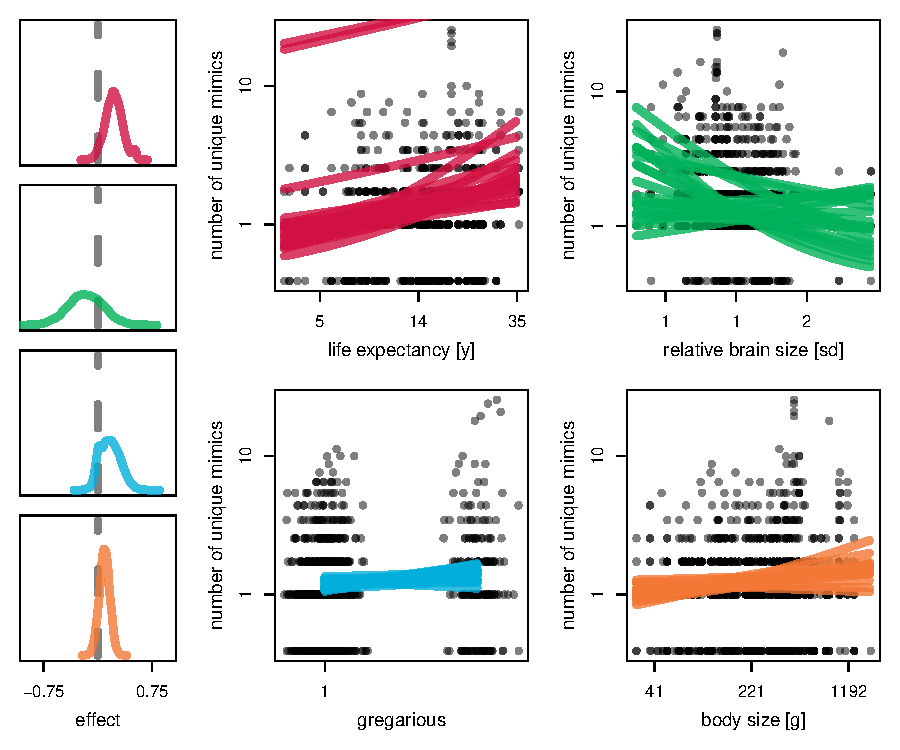
\includegraphics{/Users/ssmeele/ownCloud/Simeon/MPI AB/Side projects/Parrort mimicry/parrot_mimicry/ANALYSIS/RESULTS/results number of unique words.pdf}
\caption{Variables influencing the number of words an individual
produced in a video. Lefthand side: posterior densities of the effect of
longevity (red), relative brain size (green), gregariousness (blue) and
body size (orange). For gregariousness the contrast between a
non-gregarious and a gregarious species is shown. For all other
variables the slope is shown. Righthand side: scatterplots of the raw
data (grey) and 20 posterior predictions (coloured lines) per variable.}
\end{figure}

\end{document}
